\documentclass{article}
\usepackage{graphicx}
\usepackage{subcaption}
\graphicspath{ {./images/} }
\usepackage{float}
\usepackage{multirow}
\title{What Determines House Prices in Ames, Iowa}
\author{Bryan Klee and Joe Lucas}
\date{July 31st, 2022}
\begin{document}
	\maketitle
	\section{Abstract}
	With inflated home prices as a result of the pandemic, it is hard to tell nowadays what is the true reason for a home's value. This study set out to determine if Location, Size, Condition, Quality, and Age are the true main factors in determining a home's price. With home sales data collected from homes in Ames, Iowa between the years 2006-2010, we set out to create a model which would tell us just that. While there were many features at our disposal to explore, our goal was to answer the main question, "Do Location, Size, Condition, Quality, and Age affect home prices?" So, we did just that by only including features in this study which related to those five factors. Three different models, were produced: Multiple Linear Regression, Ridge Regression, and LASSO Regression. All three models were chosen because of their ability to predict home price, while also telling us which factors were the most important. While all three models explained about 91 percent of the variance in home price, they confirmed our suspicians. Overall Quality and Condition are the most influential factors in the price of a home, followed by Location, Size, and Age. For rankings of Quality and Condition, it is only the rankings at the ends of the spectrum (1-3 and 8-10) that affect the home's price the most. This study should be expaned to include more miscellaneous variables that might have a hidden significant effect on the price of a home. 
	
	\section{Introduction}
	Housing is one of a human's three most basic needs, so home prices will significantly affect everyone's financial health and well-being. Studies have shown, and a general knowledge of homes would tell you, that the most important factors of house price are location, quality of Materials, condition of the home, and the age of the home. We sought to determine whether these really are the most important factors, if any of these factors are more important than anotehr, or if none of those factors are important at all. 
	
	Knowing the factors that play into house prices can be useful to all different kinds of people, no matter the home owner status. Those that are looking to buy will have a better understanding of what makes the homes value and can look deeper at those important factors to make sure the house truly is the value they say it is. This can help with finding a good buy or steering you away from a bad one. For those looking to sell their house they can use this to determine the true value of their own house, or if they are looking to sell in a few years, they could properly update their home to best improve their house's value.
	
	This topic is even more relevant given the conditions of the Housing Market today. Since the pandemic, the prices of homes have been increasing exponentially. This is for a lot of reasons, some that can't be seen in the data set we are dealing with. However this analysis could be used to see the true value of homes in a non pandemic economy. This along with a current data set could be used to determine how overinflated the price of homes are compared to their true value. 
	
	\subsection{Data}
	We found a data set of house sales in Ames, Iowa between 2006 and 2010 gathered from the Ames Assessor's Office. The data includes almost any kind of attribute a house can have, ranging from how many rooms there are and the square footage of the house, to if there is a pool or garage and what type of road goes to the home. In total there were 2,930 homes sold between 2006 and 2010, each having 79 descriptive attributes. This amount of data is both helpful and hindering. With the large amount of houses and attributes it should give more accurate results, but will require more effort in cleaning the data overall and in narrowing down the data set to only the most important factors. We split the data in half, the first half as apart of a training set, and the second half as a validation set. 
	
	
	\section{Materials and Methods}
	The housing data set we have has 80 variables for each house, which include 23 nominal, 23 ordinal, 14 discrete, and 20 continuous variables. In order to get a more comprehendable data set we will have to reduce the variables to a set of features we want to look at. In order to do this we create a general category of 4 variables, and these are the four factors we think are most important, Location, Quality, Condition, and Age. Out of these 4 categories we come up with we have 12 features we come down to. These can be just variables in from our raw data or combinations of variables such as Total Square Footage, which is the sum of 1st Floor Living Area Square Footage, 2nd floor and the basement. So we trim the data set of 80 variables down to a feature group of 12 to study.

	\subsection{Initial Feature Reduction}

	A number of the features that we decided to keep were an aggregate of separate features that came in the original dataset. Those features are outlined below:

	\begin{enumerate}
		\item Total Square Footage
		\item[\textbullet] Total Basement Square Footage + General Living Area
		\item Total Porch Square Footage
		\item[\textbullet] Open Porch Square Footage + Enclosed Porch Square Footage + Three Screened In Porch Square Footage + Full Screened In Porch Square Footage
		\item Total Bathrooms
		\item[\textbullet] Full Bathrooms + Half Bathrooms
		\item Years Old
		\item[\textbullet] 2022 - Year Built
		\item Lot Frotage
		\item Lot Area
		\item Neighborhood
		\item Overall Quality
		\item Overall Condition
		\item Total Rooms Above Ground
		\item Garage Area
		\item Year Sold
		\item Month Sold
		\item Sale Price
		\item Dependent Variable
	\end{enumerate}

	\subsection{Skewness of Variables}
	 
	Initial Exploration of our features showed that many of them were strongly skewed to the right. A total of six features of the features and in order to make them normally distributed and ready for analysis we will log transform them. A plot of their distributions is shown in the figure below.
	
	\begin{figure}[H]
		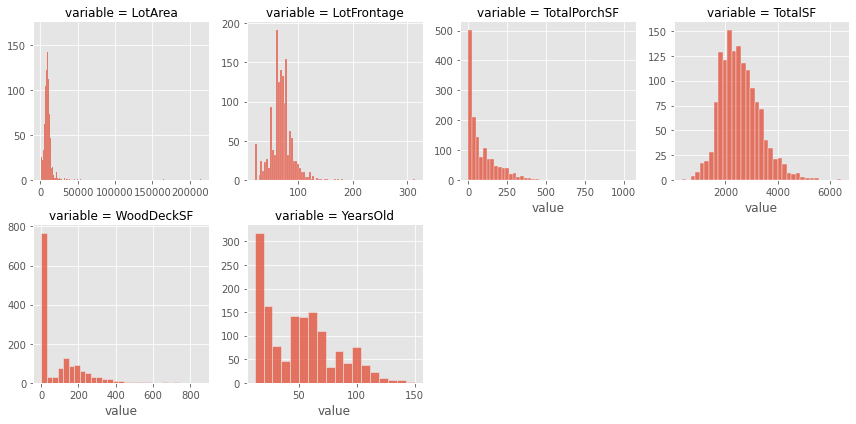
\includegraphics[width=\textwidth]{skewplots}
		\caption{Histograms for the features. Lot Area, Lot Frontage, Total Porch Square Footage, Total Square Footage, Wood Deck Square Footage, and Years Old. Their skew values are 1.54, 12.59, 1.55, 0.65, 2.01, and 0.61, respectively.}
		\label{fig:skew}
	\end{figure}
	
		
	
	Finally we have our target variable. Sale Price for the house is our target variable, as that is the ultimate outcome when looking at all the variables together. It is a pretty self explanatory variable being the price the house was sold at, as a numerical variable. Since it is our target, we want to inspect it more closely and better understand and prepare it for analysis. We can see from the bar chart that the sale price is pretty heavily skewed to the right and will need some adjustments to be made. In order to get it to a normal distribution we will log transform Sales Price.

	%...

\begin{figure}[h!]
	\centering
	\begin{subfigure}[b]{0.4\linewidth}
	  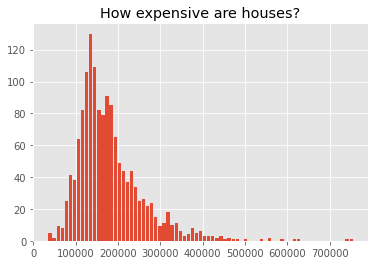
\includegraphics[width=\linewidth]{salehist}
	  \caption{A histogram of the target variable, Sale Price}
	\end{subfigure}
	\begin{subfigure}[b]{0.4\linewidth}
	  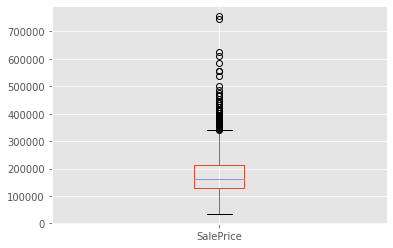
\includegraphics[width=\linewidth]{salebox}
	  \caption{A box plot of the target variable, Sale Price. }
	\end{subfigure}
	\caption{Notice the outliers in upper ranges.}
	\label{fig:saleprice}
  \end{figure}
  
  %...

  \subsection{Correlation of Variables}
	
	We then take a look at some different correlations with sale price and with all the other features. With the correlation to just sales price we see that Total Square Footage is the most positive correlated feature and Years Old is the highest negative correlated feature. This is starting to confirm what we believe and shows that Age and Size have the biggest impact on sale price. When looking at the correlation matrix, we see Total Square Footage and Total Rooms Above Ground, and Total Baths and Total Square footage are the most highly correlated features. This would make sense as the more rooms there are, the higher the square footage will be. The same holds for Total baths and square footage, as the more bathrooms the more space in the house there will be. From this, since Bathroom Square Footage is not included in Total Square Footage we will keep it, and remove Total Rooms Above Ground. These are the correlation graphs:
	
	%...

	\begin{figure}[h!]
		\centering
		\begin{subfigure}[b]{0.4\linewidth}
		  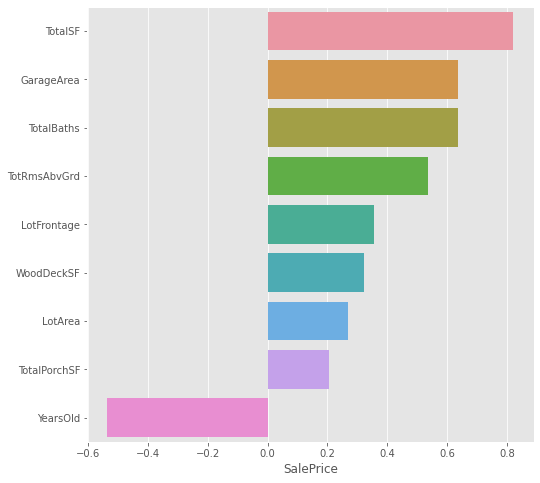
\includegraphics[width=\linewidth]{salecorr}
		  \caption{A bar plot of correlation coefficients of numerical variables to the target variable, Sale Price.}
		\end{subfigure}
		\begin{subfigure}[b]{0.4\linewidth}
		  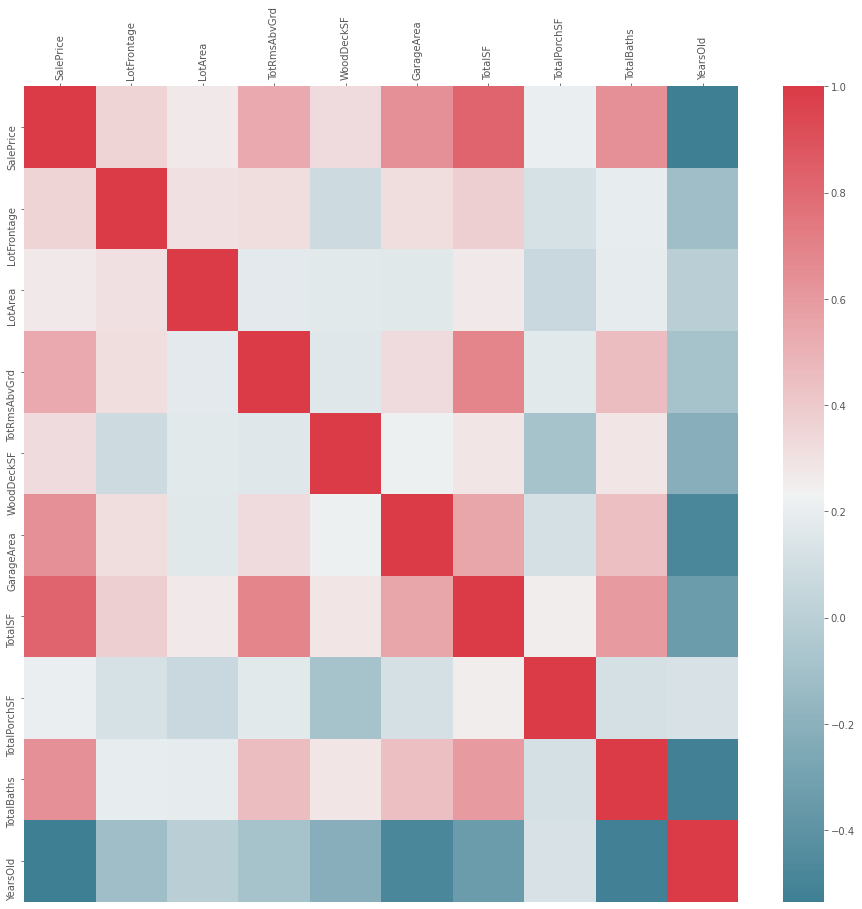
\includegraphics[width=\linewidth]{corrmatrix}
		  \caption{A correlation matrix of all numerical variables in the dataset.}
		\end{subfigure}
		\label{fig:correlation}
	  \end{figure}
	  
	  %...
	

	\subsection{Analysis of Categorical Variables}

	Looking at the categorical variables we plot the averages against each other to get a visual idea of whats going on. Visually looking at the plots, we see that Neighborhood and Overall Quality look to have statistically significant different means. 
	
	\begin{figure}[H]
		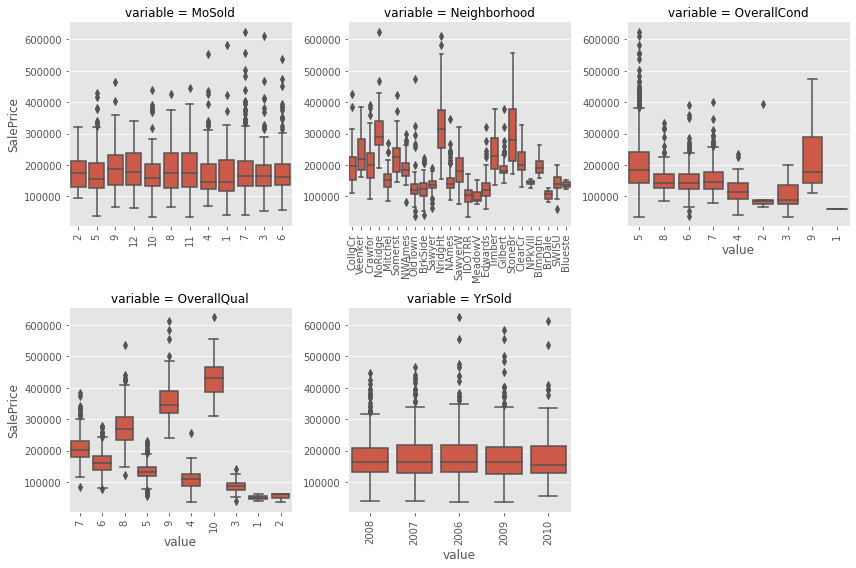
\includegraphics[width=\textwidth]{catboxes}
		\caption{Box Plots of all categorical variables. Neighborhood, Overall Qual, and Overall Condition have noticably different means.}
		\label{fig:cats}
	\end{figure}
	
	Since it appears so, we will run an ANOVA test to truly determine if our categorical values are different. After running ANOVA on all our variables we see that the only features that do not have different means are Month Sold and Year Sold. Since they do not have different means we will remove them as they have no impact. 
	
	\begin{table}[H]
		\centering
		\begin{tabular}{llll}
		\hline
		\multicolumn{1}{|l|}{Feature} & \multicolumn{1}{l|}{F-Stat} & \multicolumn{1}{l|}{P-value} & \multicolumn{1}{l|}{Significant?} \\ \hline
		Overall Quality               & 374.11                      & 0.00                         & True                              \\
		Neighborhood                  & 74.02                       & 1.63e-230                    & True                              \\
		Overall Condition             & 28.84                       & 1.87e-41                     & True                              \\
		Month Sold                    & 0.98                        & 0.458                        & False                             \\
		Year Sold                     & 0.32                        & 0.865                        & False                            
		\end{tabular}
		\end{table}
	

	Overall Quality, Neighborhoods and Overall Condition do have significantly different means and therefore they may have an impact and we will have to keep them in for analysis.

	\section{Modeling}

	\subsection{Data Prep and Standardization}
	
	As stated in previous the "Skewness of Variables" section, we first log transform the features LotFrontage, Lot Area, Wood Deck Square Footage, Total Square Footage, Total Porch Square Footage, and Years Old. In addition to those features, we log transform the target variable, Sales Price.

	\subsection{Binary Variables}

	Keep in mind that there are only three categorical variables remaining at this point: Location, Overall Quality, and Overall Condition.

	In order to pass these categorical variables into a regression model, they must be converted into binary variables. One for each member of the category. The following number of binary variables were created from each categorical features:

	\begin{enumerate}
		\item Neighborhood
		\item[\textbullet] 25: One for each neighborhood
		\item Overall Quality
		\item[\textbullet] 10: One for each rating 1 - 10.
		\item Overall Condition
		\item[\textbullet] 10: One for each rating 1 - 10.
	\end{enumerate}

	\subsection{Multi-Linear Regression}

	Our first approach will be multi-linear regression.

	With multi-linear regression, we first wanted to calculate The Variance Inflation Factor (VIF) for each variable. While we were aiming for variables with a VIF of five or less, we would accept anything VIF below ten. Each numerical variable and their VIF is shown in the table below:

	\begin{table}[H]
		\centering
		\begin{tabular}{ll}
		\hline
		\multicolumn{1}{|l|}{feature} & \multicolumn{1}{l|}{VIF} \\ \hline
		LotFrontage                   & 2.29459                  \\
		LotArea                       & 2.854278                 \\
		WoodDeckSF                    & 1.244522                 \\
		GarageArea                    & 1.997873                 \\
		TotalSF                       & 3.169309                 \\
		TotalPorchSF                  & 1.272145                 \\
		TotalBaths                    & 2.113038                 \\
		YearsOld                      & 7.157472                
		\end{tabular}
		\end{table}
		
	From the VIF scores, we have determined that we will keep all seven of the numerical features in our feature set. 

	From there it is time to perform the MLR.

	While this table is lengthy because of the 45 binary variables, you can still discern it's significance:

	\begin{table}[H]
		\centering
		\begin{tabular}{lllllll}
		\hline
		\multicolumn{1}{|l|}{Feature}    & \multicolumn{1}{l|}{coef} & \multicolumn{1}{l|}{std err} & \multicolumn{1}{l|}{t} & \multicolumn{1}{l|}{P\textgreater{}|t|} & \multicolumn{1}{l|}{{[}0.025} & \multicolumn{1}{l|}{0.975{]}} \\ \hline
		Lot Frontage                     & 0.0007                    & 0.006                        & 0.122                  & 0.903                                   & -0.011                        & 0.012                         \\
		Lot Area                         & 0.0575                    & 0.006                        & 8.991                  & 0                                       & 0.045                         & 0.07                          \\
		Wood Deck SF                     & 0.0094                    & 0.004                        & 2.221                  & 0.027                                   & 0.001                         & 0.018                         \\
		Garage Area                      & 0.0416                    & 0.005                        & 7.779                  & 0                                       & 0.031                         & 0.052                         \\
		Total SF                         & 0.1208                    & 0.007                        & 17.927                 & 0                                       & 0.108                         & 0.134                         \\
		Total Porch SF                   & 0.0165                    & 0.004                        & 3.875                  & 0                                       & 0.008                         & 0.025                         \\
		Total Baths                      & 0.0532                    & 0.006                        & 9.66                   & 0                                       & 0.042                         & 0.064                         \\
		Years Old                        & -0.0974                   & 0.01                         & -9.614                 & 0                                       & -0.117                        & -0.077                        \\
		Neighborhood Bloomington Heights & 1.9433                    & 0.035                        & 55.257                 & 0                                       & 1.874                         & 2.012                         \\
		Neighborhood Bluestem            & 1.9833                    & 0.119                        & 16.639                 & 0                                       & 1.749                         & 2.217                         \\
		Neighborhood Briardale           & 1.9228                    & 0.044                        & 44.018                 & 0                                       & 1.837                         & 2.008                         \\
		Neighborhood Brookside           & 1.9465                    & 0.023                        & 85.246                 & 0                                       & 1.902                         & 1.991                         \\
		Neighborhood Clear Creek         & 1.9423                    & 0.03                         & 64.753                 & 0                                       & 1.883                         & 2.001                         \\
		Neighborhood College Creek       & 1.8809                    & 0.016                        & 118.261                & 0                                       & 1.85                          & 1.912                         \\
		Neighborhood Crawford            & 2.0665                    & 0.023                        & 91.559                 & 0                                       & 2.022                         & 2.111                         \\
		Neighborhood Edwards             & 1.844                     & 0.017                        & 106.709                & 0                                       & 1.81                          & 1.878                         \\
		Neighborhood Gilbert             & 1.88                      & 0.021                        & 90.873                 & 0                                       & 1.839                         & 1.921                         \\
		Neighborhood IDOTRR              & 1.7453                    & 0.027                        & 64.386                 & 0                                       & 1.692                         & 1.799                         \\
		Neighborhood Meadow Village      & 1.8414                    & 0.046                        & 39.816                 & 0                                       & 1.751                         & 1.932                         \\
		Neighborhood Mitchell            & 1.839                     & 0.022                        & 84.02                  & 0                                       & 1.796                         & 1.882                         \\
		Neighborhood North Ames          & 1.8943                    & 0.014                        & 138.41                 & 0                                       & 1.867                         & 1.921                         \\
		Neighborhood  Northpark Villa    & 1.9448                    & 0.051                        & 38.343                 & 0                                       & 1.845                         & 2.044                         \\
		Neighborhood Northwest Ames      & 1.8522                    & 0.019                        & 98.438                 & 0                                       & 1.815                         & 1.889                         \\
		Neighborhood Northridge          & 2.0108                    & 0.025                        & 79.557                 & 0                                       & 1.961                         & 2.06                          \\
		Neighborhood Northridge Heights  & 1.9457                    & 0.022                        & 89.016                 & 0                                       & 1.903                         & 1.989                         \\
		Neighborhood Old Town            & 1.8132                    & 0.019                        & 95.312                 & 0                                       & 1.776                         & 1.851                         \\
		Neighborhood SWISU               & 1.9037                    & 0.038                        & 49.613                 & 0                                       & 1.828                         & 1.979                         \\
		Neighborhood Sawyer              & 1.8826                    & 0.019                        & 96.571                 & 0                                       & 1.844                         & 1.921                         \\
		Neighborhood Sawyer West         & 1.869                     & 0.021                        & 90.713                 & 0                                       & 1.829                         & 1.909                         \\
		Neighborhood Somerset            & 1.9179                    & 0.02                         & 94.582                 & 0                                       & 1.878                         & 1.958                         \\
		Neighborhood Stone Brook         & 2.036                     & 0.029                        & 69.037                 & 0                                       & 1.978                         & 2.094                         \\
		Neighborhood Timerberland        & 1.8992                    & 0.027                        & 71.258                 & 0                                       & 1.847                         & 1.951                         \\
		Neighborhood Veenker             & 1.9635                    & 0.038                        & 51.042                 & 0                                       & 1.888                         & 2.039                         \\
		Overall Quality 1                & 4.8229                    & 0.06                         & 79.72                  & 0                                       & 4.704                         & 4.942                         \\
		Overall Quality 10               & 5.1388                    & 0.041                        & 125.813                & 0                                       & 5.059                         & 5.219                         \\
		Overall Quality 2                & 4.4444                    & 0.073                        & 60.932                 & 0                                       & 4.301                         & 4.587                         \\
		Overall Quality 3                & 4.5405                    & 0.031                        & 144.574                & 0                                       & 4.479                         & 4.602                         \\
		Overall Quality 4                & 4.6315                    & 0.019                        & 243.047                & 0                                       & 4.594                         & 4.669                         \\
		Overally Quality 5               & 4.6886                    & 0.013                        & 357.467                & 0                                       & 4.663                         & 4.714                         \\
		Overall Quality 6                & 4.748                     & 0.012                        & 382.295                & 0                                       & 4.724                         & 4.772                         \\
		Overall Quality 7                & 4.8053                    & 0.013                        & 358.487                & 0                                       & 4.779                         & 4.832                         \\
		Overall Quality 8                & 4.8874                    & 0.017                        & 292.007                & 0                                       & 4.855                         & 4.92                          \\
		Overall Quality 9                & 5.0612                    & 0.026                        & 197.717                & 0                                       & 5.011                         & 5.111                         \\
		Overall Condition 1              & 4.8229                    & 0.06                         & 79.72                  & 0                                       & 4.704                         & 4.942                         \\
		Overall Condition 2              & 5.2046                    & 0.059                        & 87.627                 & 0                                       & 5.088                         & 5.321                         \\
		Overall Condition 3              & 5.1532                    & 0.032                        & 161.309                & 0                                       & 5.09                          & 5.216                         \\
		Overall Condition 4              & 5.3107                    & 0.021                        & 251.545                & 0                                       & 5.269                         & 5.352                         \\
		Overall Condition 5              & 5.3378                    & 0.011                        & 477.68                 & 0                                       & 5.316                         & 5.36                          \\
		Overall Condition 6              & 5.4137                    & 0.012                        & 434.983                & 0                                       & 5.389                         & 5.438                         \\
		Overall Condition 7              & 5.4798                    & 0.014                        & 394.074                & 0                                       & 5.453                         & 5.507                         \\
		Overall Condition 8              & 5.4771                    & 0.02                         & 280.313                & 0                                       & 5.439                         & 5.515                         \\
		Overall Condition 9              & 5.5687                    & 0.033                        & 169.276                & 0                                       & 5.504                         & 5.633                        
		\end{tabular}
		\end{table}

	From the above table, we can see that in general, the model is pretty effective. With an Adjusted R-Squared of 0.909, we are explaining almost 91 percent of the variance. Our plot of residuals may be slightly skewed to the positive residuals, but nothing of too much concern. The p-value of the model was too low for the software to discern, so we are left with a p-value that is virtually 0. 

	\begin{figure}[H]
		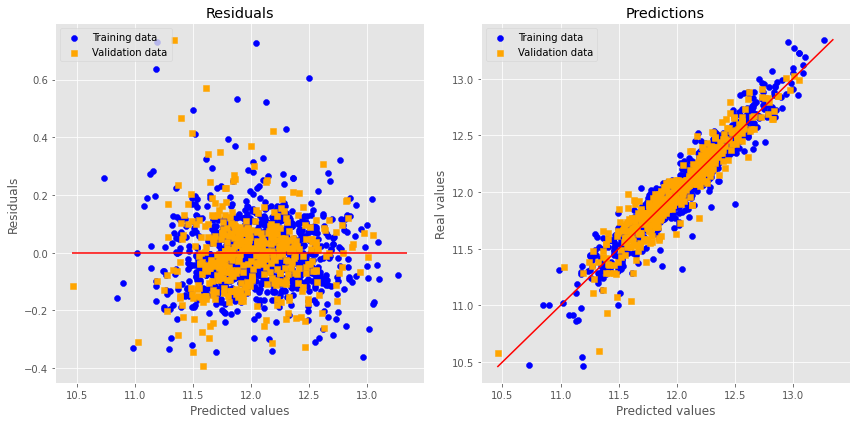
\includegraphics[width=\textwidth]{mlrplot}
		\caption{Residual Plots for Multiple Linear Regression}
		\label{fig:skew}
	\end{figure}

	\subsection{Ridge Regression}

	While the outputs from our Multiple Linear Regression were encouraging, we knew there were more techniques that would help us understand the true relationship between home qualities and the home's price. The first of those other techniques is Ridge Regression.
	Ridge Regression is a shrinkage method that's goal is to weigh coefficients by introducing a shrinkage penalty. This shrinkage penalty adds a small amount of bias that, in essence, shrinks some of the coefficients asymptotically closer and closer to 0. In many cases, not only will it give you a more accurate model on unknown data, it will inform you on which of your coefficients are the most influential on your dependent variable. The formula for ridge regression is below:

	\begin{figure}[H]
		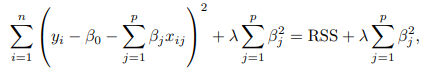
\includegraphics[width=\textwidth]{ridgeform}
		\caption{Formula for Ridge Regression. Is the same as OLS Regression, but a shrinkage penalty is applied.}
		\label{fig:skew}
	\end{figure}

	In order to choose the value for our tuning parameter, we decided to run a 5-Fold Cross validation. After performing said cross validation, it was determined that the best alpha level for the Ridge Regression model was 0.7. After performing ridge regression, here was our output, as well as the features who's coefficients were given the most weight:

	%...

	\begin{figure}[h!]
		\centering
		\begin{subfigure}[b]{0.4\linewidth}
		  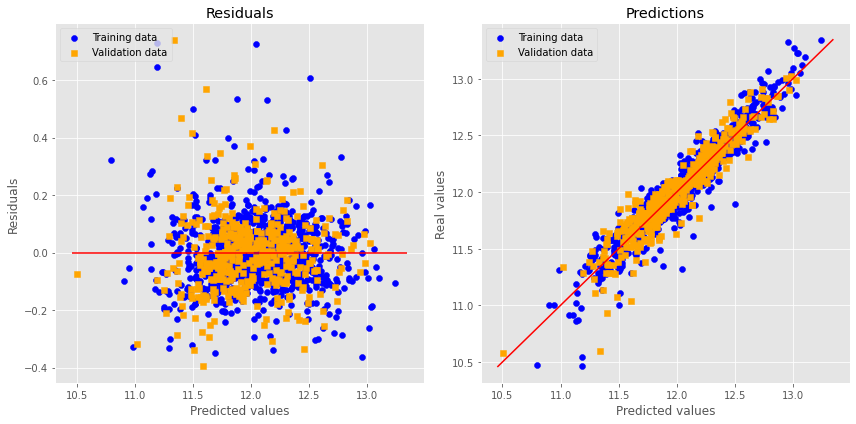
\includegraphics[width=\linewidth]{ridgeplot}
		  \caption{Residual Plots for Ridge Regression}
		\end{subfigure}
		\begin{subfigure}[b]{0.4\linewidth}
		  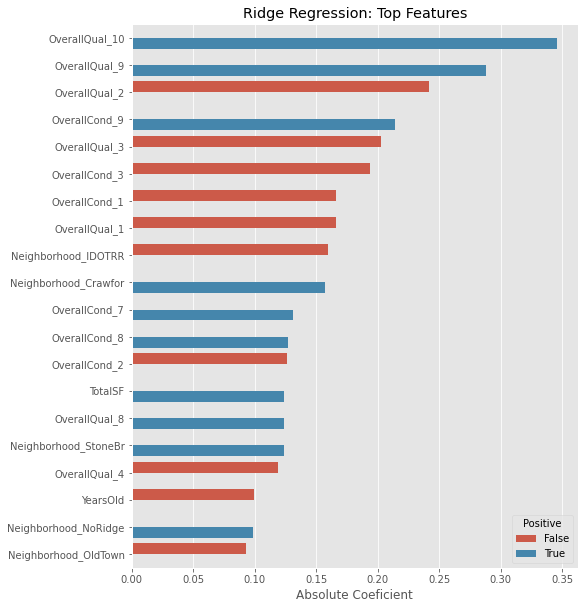
\includegraphics[width=\linewidth]{ridgefeat}
		  \caption{Most heavy feature weights as a result of Ridge Regression}
		\end{subfigure}
		\label{fig:correlation}
	  \end{figure}
	  
	  %...

	After performing Ridge Regression, we were able to increase our Adjusted R-Squared only slightly, to 0.9103. However, what we gain more insight from is the variable's that it weighs the most heavily. Those features were almost all measure of Quality and Condition. The rankings at the top and bottom of the spectrum, 1, 2, 9, and 10, were given the most weight. 

	\subsection{LASSO Regression}

	The last model we used against this dataset was a LASSO regression model. A LASSO Regression is similar Ridge Regression in the sense that it is a shrinkage method. Weights are also applied to coefficients, but unlike Ridge, LASSO is able to shrink "meaningless" coefficients all the way down to 0. So in a sense, it is a form of subset selection. The formula for LASSO Regression is:

	\begin{figure}[H]
		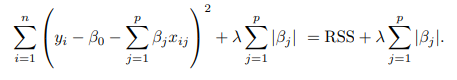
\includegraphics[width=\textwidth]{lassoform}
		\caption{Formula for LASSO Regression. Is the same as OLS Regression, but a shrinkage penalty is applied.}
		\label{fig:skew}
	\end{figure}

	In order to choose the value for our tuning parameter, we decided to run a 5-Fold Cross validation. After performing said cross validation, it was determined that the best alpha level for the LASSO Regression model was 5e-05. After performing LASSO Regression, here was our output, as well as the features who's coefficients were given the most weight:

	%...

	\begin{figure}[h!]
		\centering
		\begin{subfigure}[b]{0.4\linewidth}
		  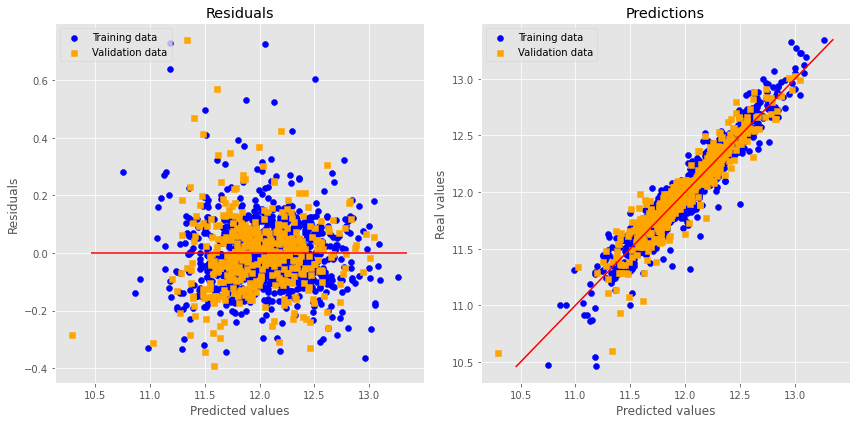
\includegraphics[width=\linewidth]{lassoplot}
		  \caption{Residual Plots for Lasso Regression}
		\end{subfigure}
		\begin{subfigure}[b]{0.4\linewidth}
		  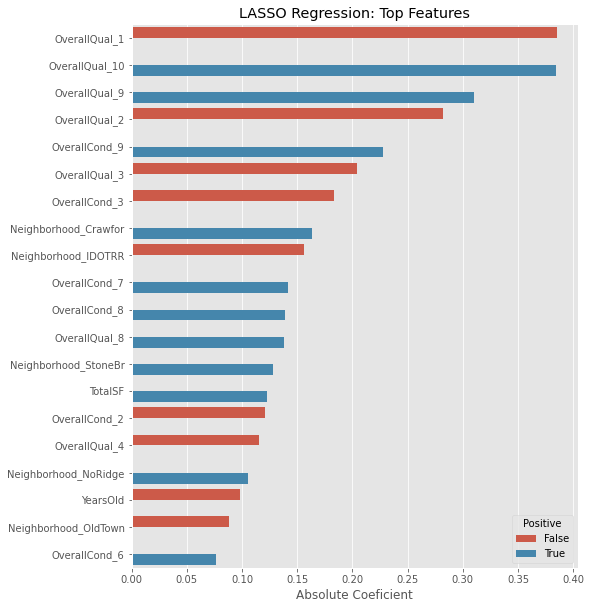
\includegraphics[width=\linewidth]{lassofeat}
		  \caption{Most heavy feature weights as a result of LASSO Regression}
		\end{subfigure}
		\label{fig:correlation}
	  \end{figure}
	  
	  %...

	The LASSO Regression model dropped 3 of the 52 features, those being: Lot Frontage, Neighborhood SWISU, and Overall Condition 5. This comes as no surprise as again the most highly weighted features were the Overall Quality and Overall Condition scores at each end of the rating scale. Additionally, recall that the MLR found that Lot Frontage was not significant, so that could explain why LASSO reduced it to 0.

	The Adjusted R-Squared produced by the LASSO Regression was 0.9101.
	
	
	\section{Results}
	
	From our three models, we can conclude that the Ridge Regression performed the best of the 3. See the table below for the Adjusted-R Squared values for each model. Additionally, we see that the least important variable that we passed into each model was Lot Frontage.
	From the Ridge and LASSO regressions, we can see that Overall Condition, and Overall Quality are the most important factors in determining the price of a home. What's interesting, is that it is only the ratings for Condition and Quality at the top and bottom ends of the spectrum that are given any weight. This must mean that if you are willing to rate a house very poorly for Quality and Condition, it's price will almost assuredly be less. If you are blown away by the home and willing to rate it a 9 or a 10, it will assuredly cost more. However, the more "average" ratings, let's say 3-7, do not influence the price of a home as severly. It is also important to note that the old adage of "Location, Location, Location" does seem to be true as Locations were the coefficients with the third highest weighting in both the Ridge and LASSO regressions. 
	
	
	\section{Conclusion}

	We set out to prove whether Size, Condition, Quality, Location, and Age were actually significant factors in the price of a home. It is clear that these variables are indeed the main factors in determining home prices. Quality, then Condition, and then Location are the most influential. Because we reduced the original data set, it might be beneficial to redo this study with more features. While this make the models less interpretable, there may be other important factors that influence home prices that we have not thought of. In addition, expanding this study to include more homes in more locations. What affects home prices could be largely regional. For all we know, it could change from town to town, nevermind state to state or country to country. Nonetheless, it would appear that Quality, Condition, Size, and Age are the driving factors in home price. 
	
	
\end{document}